\section{Language generation and summarization}
\begin{itemize}
	\item Most tasks/methods until now have concentrated on language analysis. Next coming: tasks where we have to generate text
	\item Generation mostly has the starting point at semantic representation like distributional semantics or hidden representation for neural networks
	\item We can also concentrate on \textit{regeneration} where we convert input to another representation. Examples include summarization, translation, ...
	\item For generation, there are various subtasks (e.g. content selection, discourse structuring, ...)
	\item Approaches for generation include:
	\begin{itemize}
		\item \textit{Templates}: fixed text that has slots that can be filled
		\item \textit{Statistical}: using machine learning
		\item \textit{Deep Learning}: using deep embeddings, especially for regeneration task
	\end{itemize}
\end{itemize}
\subsection{Text Summarization}
\begin{itemize}
	\item Task: generate short version of input text with important points
	\item We distinguish between \textbf{single-document summarization} (given a single document, produce summary with important points) and \textbf{multi-document summarization} (given a set of documents, produce brief summary of combination)
	\item Also, we differentiate between \textbf{generic summarization} (identifying important parts by itself and present these) and \textbf{query-focused summarization} (regarding a query/question from the user, find relevant parts in the document/s)
	\item There are mostly main approaches:
	\begin{itemize}
		\item \textbf{Extractive summarization}: extract important info from document by copying sentences and combine them into a summary
		\item \textbf{Abstractive summarization}: interpret content of document and generate completely new sentences (much harder task!)
	\end{itemize}
	\item Most approaches deal with extractive summarization as it is much easier to realize and achieves better results till now
\end{itemize}
\subsubsection{Extractive summarization}
\begin{itemize}
	\item For extractive summarization, there are three main steps:
	\begin{enumerate}
		\item \textbf{Content selection}: identify important parts/sentences from the document 
		\item \textbf{Information ordering}: order the sentence within the summary
		\item \textbf{Sentence realization}: optimizing the text by e.g. sentence simplification
	\end{enumerate}
	\item Approaches for \textit{content selection}
	\begin{itemize}
		\item \textit{Unsupervised}: 
		\begin{itemize}
			\item Take those words that are significantly more often used than in other documents in average $\Rightarrow$ these are the ``informative'' words and mostly biased towards names/cities (pronoun resolution important to find these references as well)
			\item Measured by metrics like \texttt{tf-idf}
		\end{itemize}
		\item \textit{Supervised}:
		\begin{itemize}
			\item Large training corpus with human summary needed
			\item Sentences of summary are aligned with those in the original document, and features are extracted (position in document, sentence length, informative words, ...)
			\item Based on these features, we train a binary classifier whether a sentence should be included in the summary or not
			\item Problem: expensive to generate all this data, and the supervised approaches did not significantly outperform the unsupervised ones
		\end{itemize}
	\end{itemize}
	\item Approaches for \textit{information ordering}:
	\begin{itemize}
		\item For a single document, the sentences are mostly structured in the order they occur in the original document
	\end{itemize}
\end{itemize}
\subsubsection{Query-focused multi-document summarization}
\begin{itemize}
	\item For query-focused multi-document summarization, we need to extend the extractive summarization by two pre-processing steps:
	\begin{enumerate}
		\item Find a set of relevant documents
		\item (Optionally) simplify sentences in the documents (to make the task of content selection easier)
		\item \textit{Content selection}: identify informative sentences in the documents (much harder than for the single-document task)
		\item \textit{Information ordering}: order the sentences in the summary
		\item \textit{Sentence realization}: modify sentences to get consistent summary
	\end{enumerate}
	\item Approaches for \textit{sentence simplification}
	\begin{itemize}
		\item Parse sentences and apply hand-rules what parts of a sentence we might drop (initial adverbials as ``for example'', irrelevant attribute clauses, ...)
		\item Also possible to train a classifier to identify satellites (non-informative parts on a nucleon phrase)
	\end{itemize}
	\item Approaches for \textit{content selection} for multiple documents
	\begin{itemize}
		\item We can either combine all documents into one, or retrieve information from all documents separately and weight these documents
		\item Estimate informativeness similarly to single-document
		\item Then, start by adding the most informative sentences in summary (one by one) until the maximum length of the summary is reached
		\item When adding new sentences, we need to make sure that not the same/very similar sentences from different documents are added $\Rightarrow$ \textbf{Maximum marginal relevance}
		\begin{itemize}
			\item Iterative method to determine best sentence to add to summary. Relies on two counter-part measures:
			\item \textit{Relevance to query}: high cosine similarity between a sentence and the query indicates a high relevance for the summary
			\item \textit{Novelty regarding the summary so far}: low cosine similarity between sentences and summary
			\item Estimated score is calculated as follows (for query $Q$, summary $S$, documents $D$):
			$$\hat{s} = \arg\max_{s_i \in D} \left[\lambda \text{sim}\left(s_i, Q\right) - \left(1 - \lambda\right)\max_{s_j \in S}\text{sim}\left(s_i, s_j\right)\right]$$
		\end{itemize}
	\end{itemize}
	\item Approaches for \textit{sentence ordering}
	\begin{itemize}
		\item \textit{Chronologically}: for example by date of document
		\item \textit{Coherence}: sentences that are similar/discuss same entity should be grouped together in the summary
		\item \textit{Topical ordering}: learns set of topics present in documents (by e.g. topic modeling), and then order the sentences by topic
	\end{itemize}
\end{itemize}
\subsubsection{Summarization using neural networks}
\begin{itemize}
	\item We can apply neural networks for the task of summarization
	\item For extractive summarization, we train a RNN on word level creating a representation of words, and a RNN on sentence/document level that combines sentence embeddings
	\item Apply classifier on output of all document-level RNN to decide whether to include sentence in summary or not (problem: still captures coarse-grained features)
	\begin{figure}[ht]
		\centering
		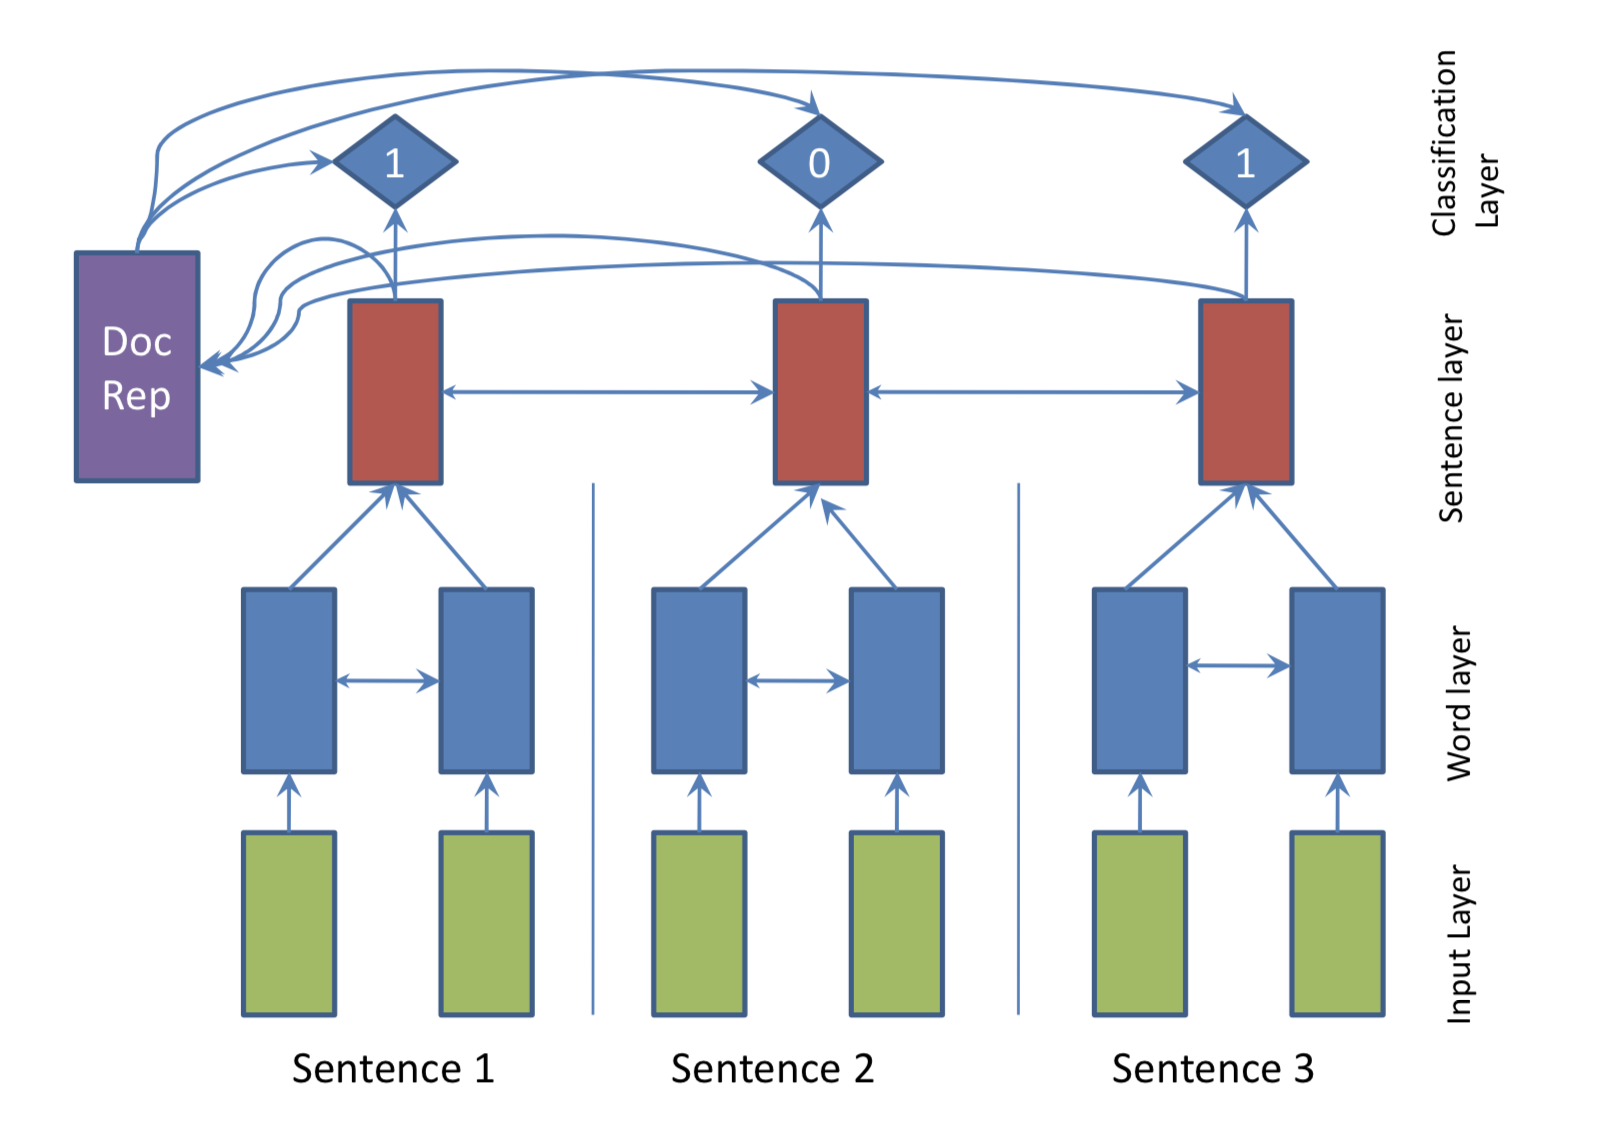
\includegraphics[width=0.3\textwidth]{figures/summarization_rnn.png}
		\caption{Summarization by RNNs}
		\label{fig:summarization_rnn}
	\end{figure}
	\item Abstractive summarization can be realized by large newspaper datasets where for a small article, a headline must be predicted
	\item We use an Encoder-Decoder architecture (seq2seq models) where the encoder generates fixed-size embedding, and the decoder generates word-by-word output given this representation (decoder is autoregressive as it takes own output back as input for next time step)
\end{itemize}
\subsubsection{Evaluating summarization models}
\begin{itemize}
	\item Human judgments of quality is too expensive
	\item Better, automatic method: \textbf{ROUGE} (recall oriented understudy for gisting evaluation)
	\item We compare a few human-generated summaries $R_1, ..., R_N$ with the system generated summary $S$ by computing the percentage of $n$-grams from the reference summaries $R_1,...,R_N$ that occur in $S$. Example: ROUGE-2 (using bigram):
	$$\frac{\sum_{R_i}\sum_{bigram_j\in R_i} \text{count}_{\text{match}}(j,S)}{\sum_{R_i}\sum_{bigram_j\in R_i} \text{count}(j, R_i)}$$
	\item Note that summary length is not considered here 
	\item Example for calculating ROUGE metric:
	\begin{figure}[ht]
		\centering
		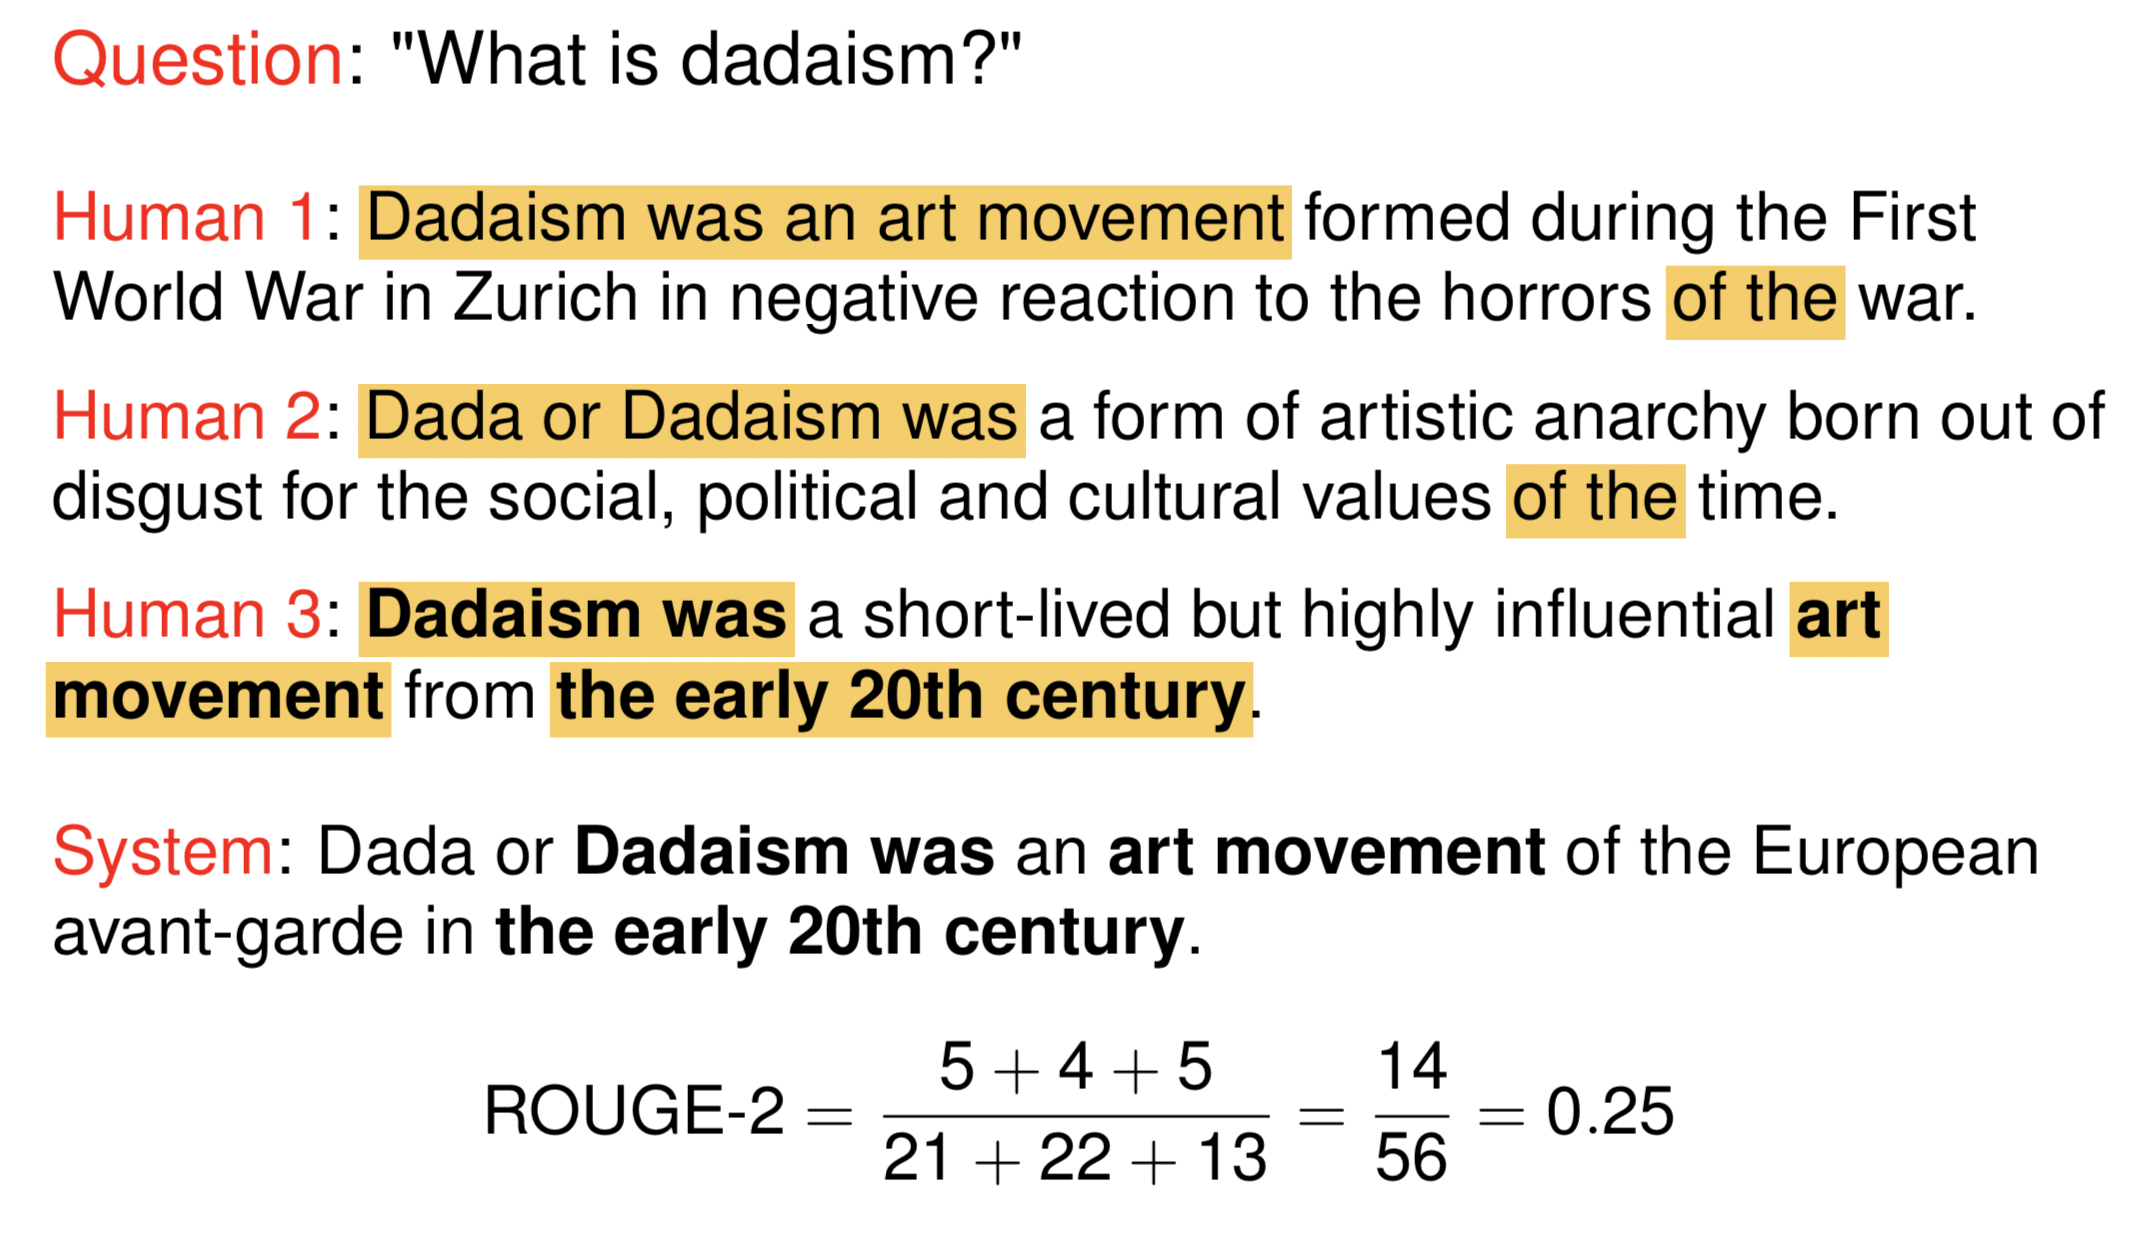
\includegraphics[width=0.5\textwidth]{figures/summarization_rogue_example.png}
		\label{fig:summarization_rogue_example}
	\end{figure}
	% summarization_rogue_example.png
\end{itemize}